The wheel shown below consists of two circles and five spokes, with a label at each point where a spoke meets a circle. A bug walks along the wheel, starting at point \(A\). At every step of the process, the bug walks from one labeled point to an adjacent labeled point. Along the inner circle the bug only walks in a counterclockwise direction, and along the outer circle the bug only walks in a clockwise direction. For example, the bug could travel along the path \(AJABCHCHIJA\), which has \(10\) steps. Let \(n\) be the number of paths with \(15\) steps that begin and end at point \(A\). Find the remainder when \(n\) is divided by \(1000\).

\begin{center}
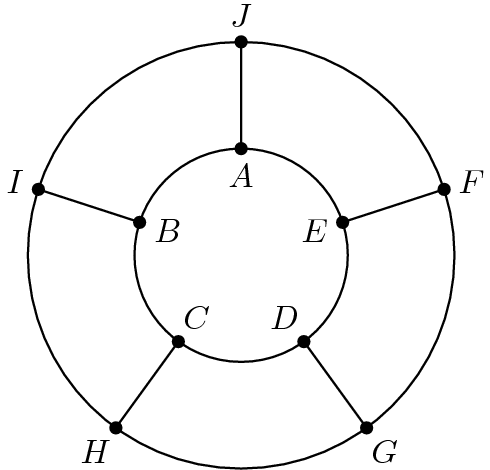
\includegraphics[width = 49.0mm]{img/fig0.png}
\end{center}